\documentclass[11pt]{article}
\usepackage[textwidth=18.0cm, textheight=23.0cm, top=2.0cm]{geometry}
\usepackage{pst-all}
\usepackage{amssymb}
\usepackage{tikz}
\usepackage{underscore}\begin{document}
\pagestyle{empty}


ClassName: \underline{\textbf{Class_03.2bp-3}}
\par
BinSize: \underline{\textbf{40 × 40}}
\par
ReduceSize: \underline{\textbf{40 × 40}}
\par
TypeNum: \underline{\textbf{20}}
\par
Num: \underline{\textbf{20}}
\par
OutS: \underline{\textbf{6400}}
\par
InS: \underline{\textbf{4964}}
\par
Rate: \underline{\textbf{0.776}}
\par
UB: \underline{\textbf{4}}
\par
LB0: \underline{\textbf{4}}
\par
LB: \underline{\textbf{4}}
\par
LBWithCut: \underline{\textbf{4}}
\par
NodeCut: \underline{\textbf{0}}
\par
ExtendedNodeCnt: \underline{\textbf{1}}
\par
GenNodeCnt: \underline{\textbf{1}}
\par
PrimalNode: \underline{\textbf{0}}
\par
ColumnCount: \underline{\textbf{4}}
\par
TotalCutCount: \underline{\textbf{0}}
\par
RootCutCount: \underline{\textbf{0}}
\par
LPSolverCnt: \underline{\textbf{1}}
\par
PricingSolverCnt: \underline{\textbf{0}}
\par
BranchAndBoundNum: \underline{\textbf{1}}
\par
isOpt: \underline{\textbf{true}}
\par
TimeOnInitSolution: \underline{\textbf{600.000 s}}
\par
TimeOnPrimal: \underline{\textbf{0.000 s}}
\par
TimeOnPricing: \underline{\textbf{0.000 s}}
\par
TimeOnRmp: \underline{\textbf{0.047 s}}
\par
TotalTime: \underline{\textbf{600.297 s}}
\par
\newpage


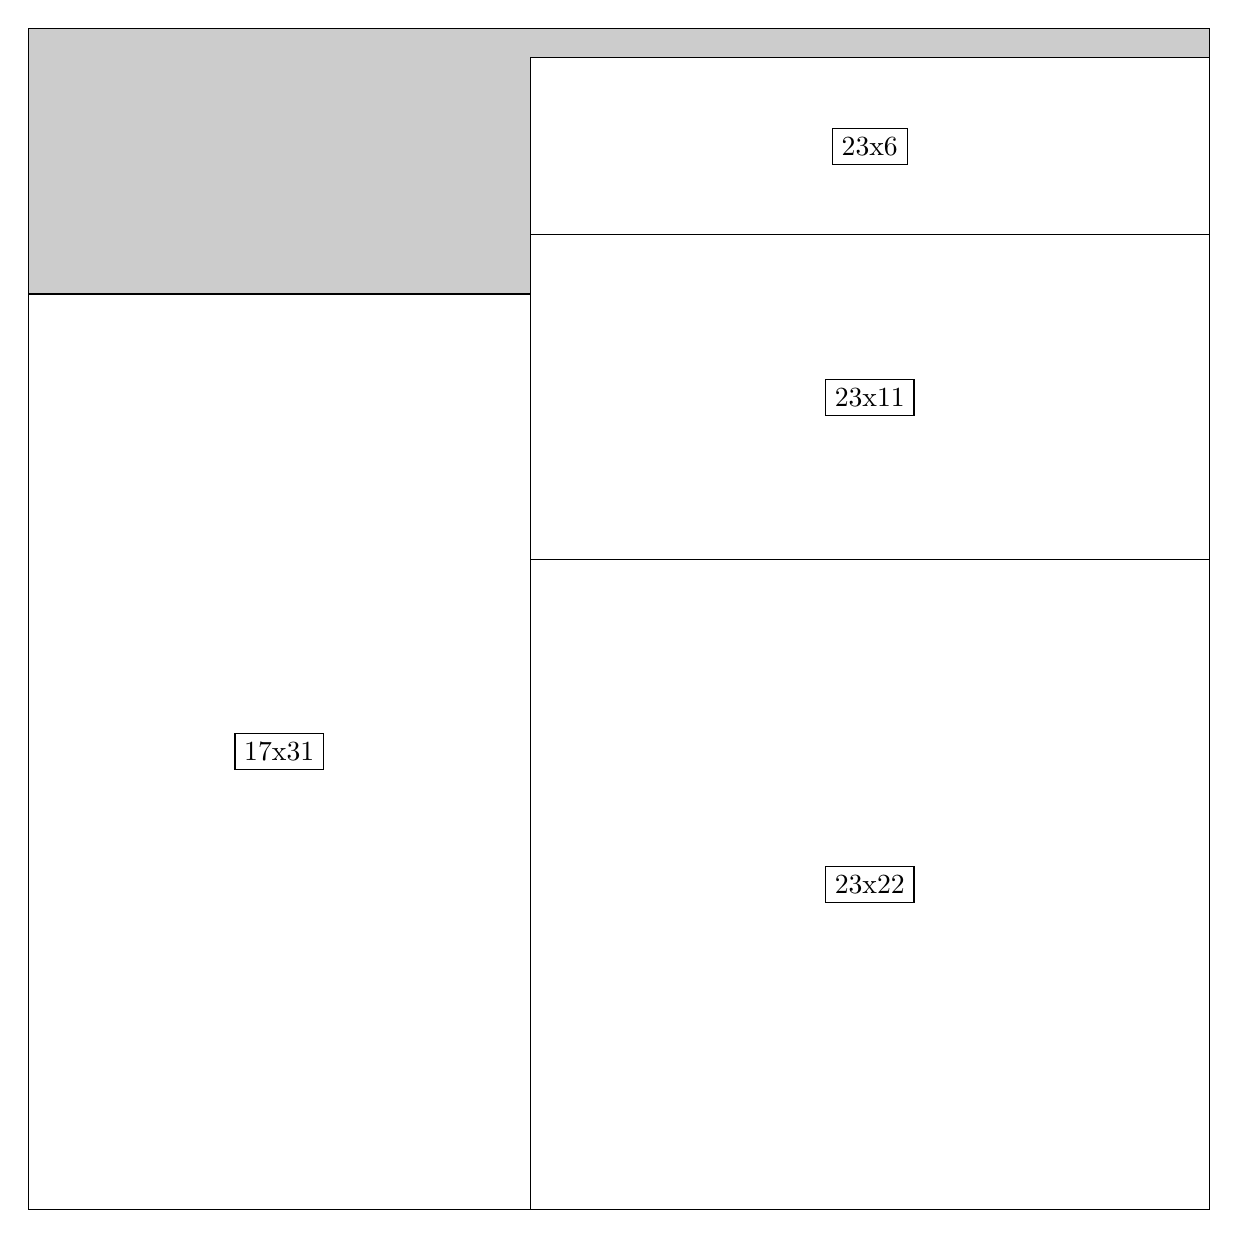
\begin{tikzpicture}[shorten >=1pt,scale=1.0,every node/.style={scale=1.0},->]
\tikzstyle{vertex}=[circle,fill=black!25,minimum size=14pt,inner sep=0pt]
\filldraw[fill=gray!40!white, draw=black] (0,0) rectangle (15.0,15.0);
\foreach \name/\x/\y/\w/\h in {23x22/6.375/0.0/8.625/8.25,23x11/6.375/8.25/8.625/4.125,23x6/6.375/12.375/8.625/2.25,17x31/0.0/0.0/6.375/11.625}
\filldraw[fill=white!40!white, draw=black] (\x,\y) rectangle node[draw] (\name) {\name} ++(\w,\h);
\end{tikzpicture}


w =23 , h =22 , x =17 , y =0 , v =506
\par
w =23 , h =11 , x =17 , y =22 , v =253
\par
w =23 , h =6 , x =17 , y =33 , v =138
\par
w =17 , h =31 , x =0 , y =0 , v =527
\par
\newpage


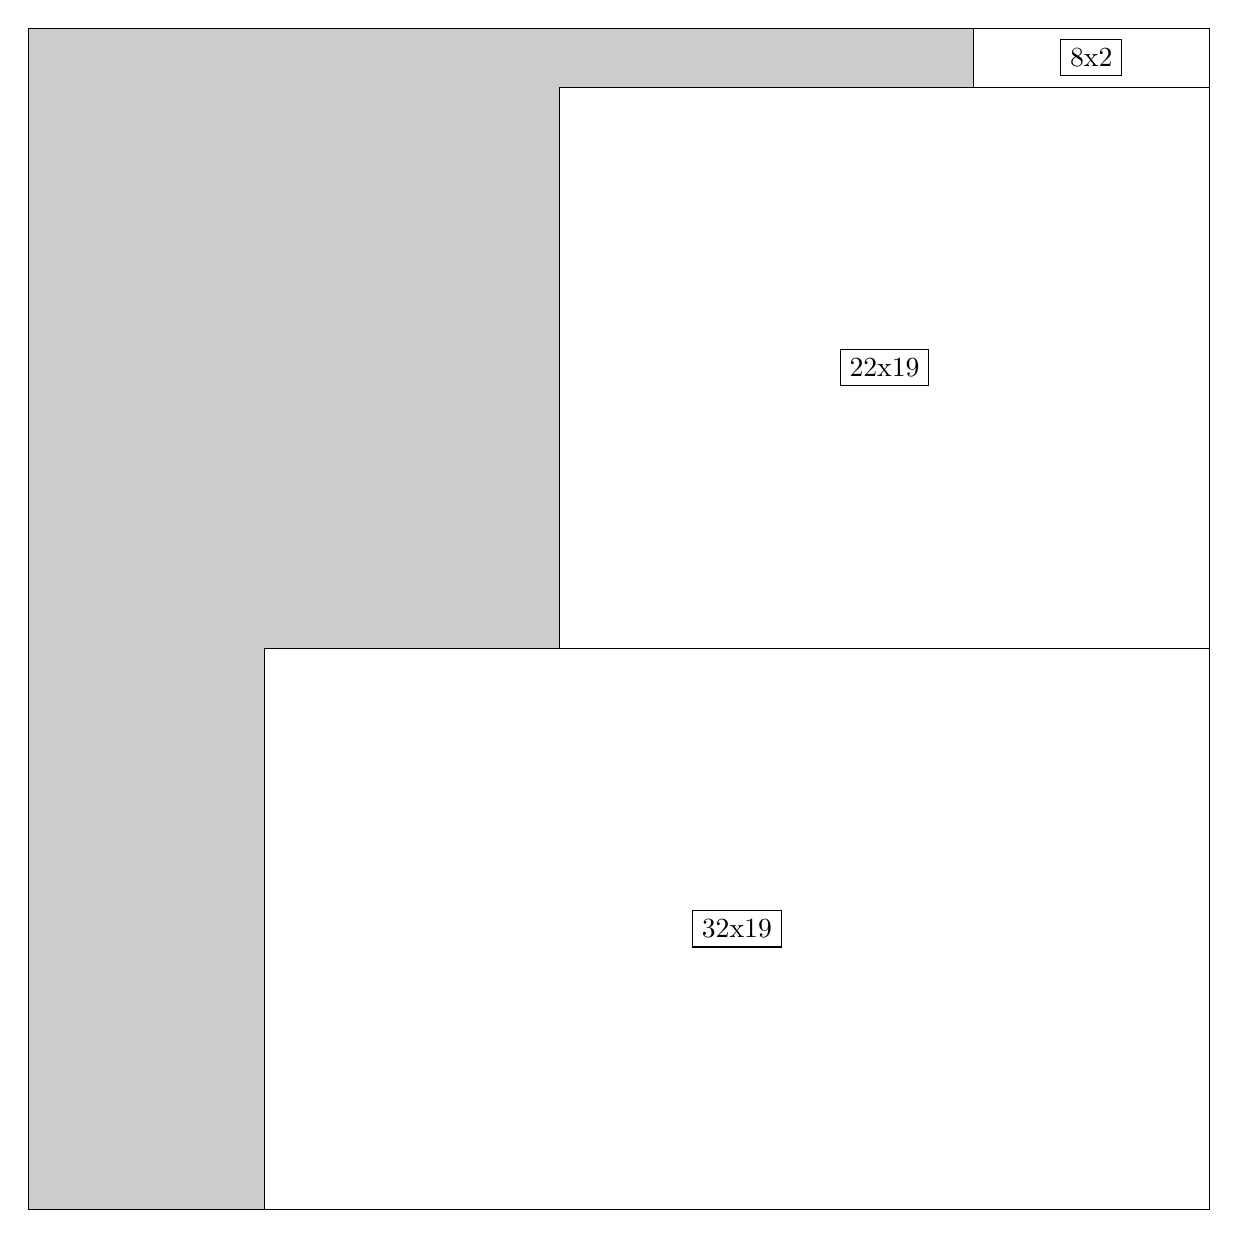
\begin{tikzpicture}[shorten >=1pt,scale=1.0,every node/.style={scale=1.0},->]
\tikzstyle{vertex}=[circle,fill=black!25,minimum size=14pt,inner sep=0pt]
\filldraw[fill=gray!40!white, draw=black] (0,0) rectangle (15.0,15.0);
\foreach \name/\x/\y/\w/\h in {32x19/3.0/0.0/12.0/7.125,22x19/6.75/7.125/8.25/7.125,8x2/12.0/14.25/3.0/0.75}
\filldraw[fill=white!40!white, draw=black] (\x,\y) rectangle node[draw] (\name) {\name} ++(\w,\h);
\end{tikzpicture}


w =32 , h =19 , x =8 , y =0 , v =608
\par
w =22 , h =19 , x =18 , y =19 , v =418
\par
w =8 , h =2 , x =32 , y =38 , v =16
\par
\newpage


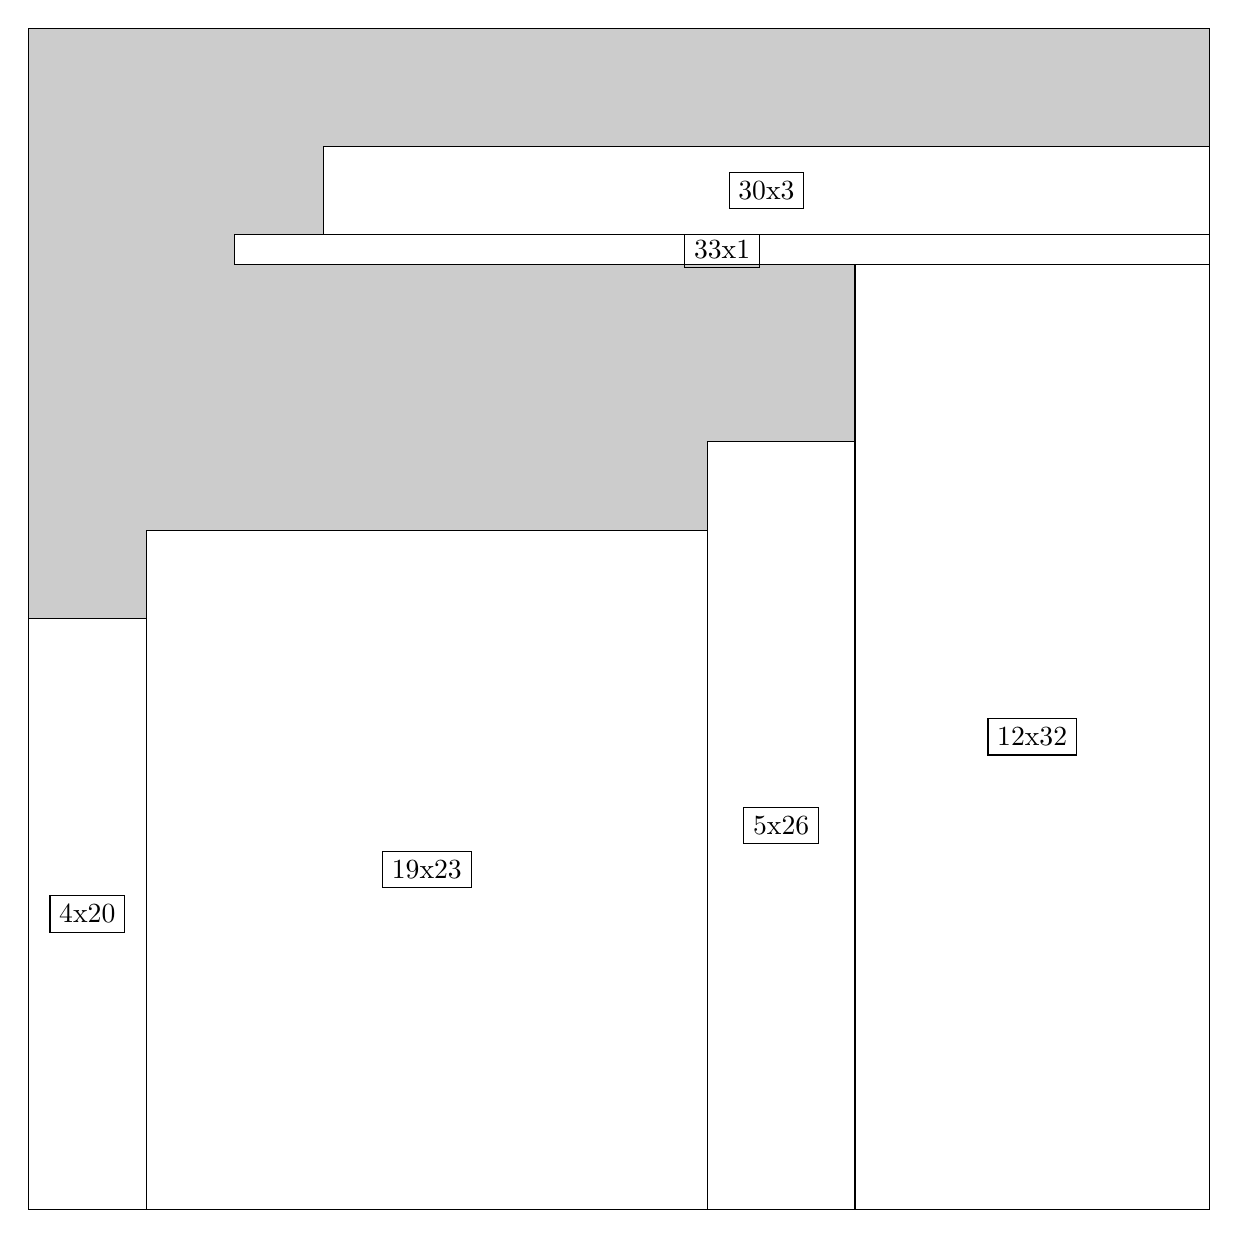
\begin{tikzpicture}[shorten >=1pt,scale=1.0,every node/.style={scale=1.0},->]
\tikzstyle{vertex}=[circle,fill=black!25,minimum size=14pt,inner sep=0pt]
\filldraw[fill=gray!40!white, draw=black] (0,0) rectangle (15.0,15.0);
\foreach \name/\x/\y/\w/\h in {12x32/10.5/0.0/4.5/12.0,5x26/8.625/0.0/1.875/9.75,19x23/1.5/0.0/7.125/8.625,4x20/0.0/0.0/1.5/7.5,33x1/2.625/12.0/12.375/0.375,30x3/3.75/12.375/11.25/1.125}
\filldraw[fill=white!40!white, draw=black] (\x,\y) rectangle node[draw] (\name) {\name} ++(\w,\h);
\end{tikzpicture}


w =12 , h =32 , x =28 , y =0 , v =384
\par
w =5 , h =26 , x =23 , y =0 , v =130
\par
w =19 , h =23 , x =4 , y =0 , v =437
\par
w =4 , h =20 , x =0 , y =0 , v =80
\par
w =33 , h =1 , x =7 , y =32 , v =33
\par
w =30 , h =3 , x =10 , y =33 , v =90
\par
\newpage


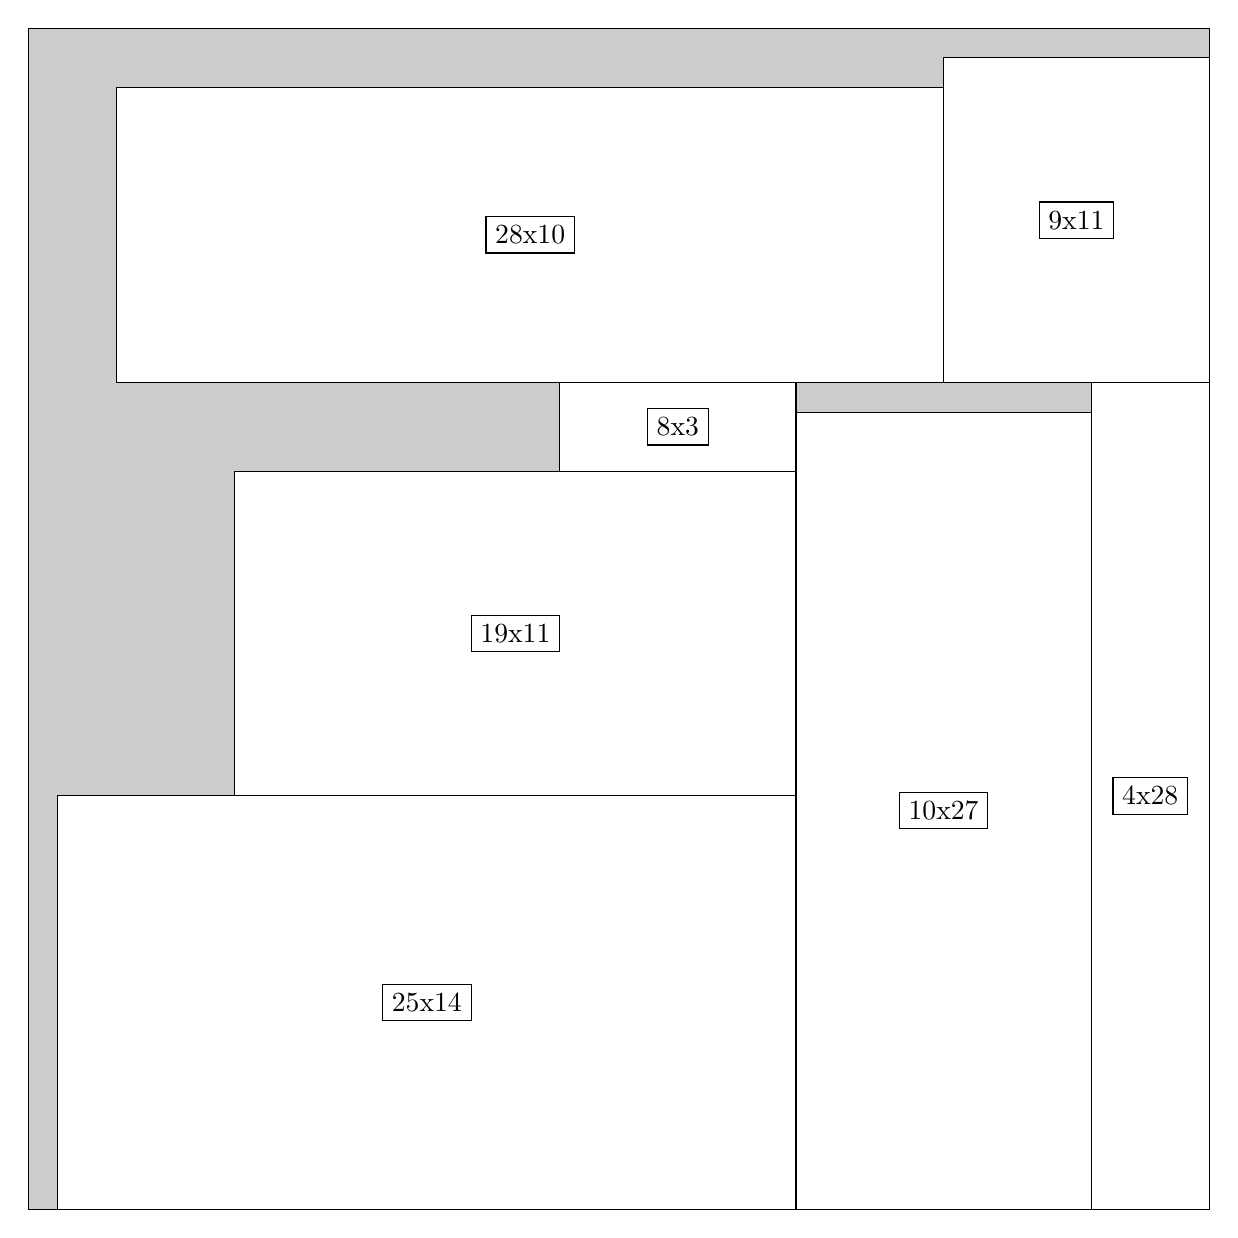
\begin{tikzpicture}[shorten >=1pt,scale=1.0,every node/.style={scale=1.0},->]
\tikzstyle{vertex}=[circle,fill=black!25,minimum size=14pt,inner sep=0pt]
\filldraw[fill=gray!40!white, draw=black] (0,0) rectangle (15.0,15.0);
\foreach \name/\x/\y/\w/\h in {4x28/13.5/0.0/1.5/10.5,10x27/9.75/0.0/3.75/10.125,25x14/0.375/0.0/9.375/5.25,19x11/2.625/5.25/7.125/4.125,8x3/6.75/9.375/3.0/1.125,9x11/11.625/10.5/3.375/4.125,28x10/1.125/10.5/10.5/3.75}
\filldraw[fill=white!40!white, draw=black] (\x,\y) rectangle node[draw] (\name) {\name} ++(\w,\h);
\end{tikzpicture}


w =4 , h =28 , x =36 , y =0 , v =112
\par
w =10 , h =27 , x =26 , y =0 , v =270
\par
w =25 , h =14 , x =1 , y =0 , v =350
\par
w =19 , h =11 , x =7 , y =14 , v =209
\par
w =8 , h =3 , x =18 , y =25 , v =24
\par
w =9 , h =11 , x =31 , y =28 , v =99
\par
w =28 , h =10 , x =3 , y =28 , v =280
\par
\newpage


\end{document}